\chapter{Methods}
\label{chap:methods}

As discussed in \autoref{chap:introduction}, the system developed in this thesis follows a pipeline consisting of two steps:
\begin{enumerate}
    \item \textbf{Object Proposal}: detection of all the logos in the image
    \item \textbf{Classification}: recognize each logo
\end{enumerate}
The first step regarding the detection of logos in the image is done by YOLO (see \autoref{sec:yolo}), while the actual recognition of the logo is performed by the classifier in an incremental learning setup. The pipeline of the system is shown in \autoref{fig:roi_and_classification}.

\begin{figure}%
	\centering

    \begin{center}
        \includegraphics[width=\columnwidth]{images/roi+classification.drawio.png}
    \end{center}

	\caption{Pipeline of the system: the class-agnostic logo detector generates ROIs, then the classification is performed by the CIL classifier.}%
	\label{fig:roi_and_classification}%
\end{figure}

The detector used in the first step is a class-agnostic logo detector: it is a logo detector since we are not interested in the detection of objects other than logo; and it is class-agnostic since the number of detected classes is only one. In fact, in this first step the detector will be responsible for finding any generic logo (i.e., a single class) in the image. This is a crucial step if we seek to achieve incremental learning logo recognition, because in this way it is possible to decouple the detection from the recognition. If the logo detector localize any generic logo in the image, and delegates the actual recognition to the CIL classifier, there is no need to develop an incremental learning detector as well.


An important aspect of the classifier is the model size in terms of number of parameters. A big model comes with several disadvantages like longer time for the training phase, higher memory requirements and longer time to make inference. To this reason, a part of this work aims to decrease the number of parameters of the classifier using two different techniques. The first technique is described in \autoref{sec:method-pruning}, using masking and pruning described in \autoref{sec:masking-pruning} it aims to prune the model after the training of each incremental step, thus reducing the number of parameters. The second approach is the Knowledge Distillation (KD) described in \autoref{sec:method-kd}, where a smaller model is trained from scratch with the supervision of a bigger model trained on the same task.

The code developed in this thesis is available in the GitHub repository\footnote{GitHub repository relative to the code of developed in this thesis: \\ \href{https://github.com/gianlucagiudice/logo-detection-recognition}{https://github.com/gianlucagiudice/logo-detection-recognition}} linked below. The system has been developed using the Python programming language, and the code is implemented using PyTorch \cite{paszke2019pytorch}, a widely use deep learning framework. The training of the models is done using the NVIDIA Tesla K80 GPU with 12GB of memory.


\vspace{1.5\baselineskip}
This chapter describes all the details about the logo detector in \autoref{sec:method-roi} and continues with the classifier in \autoref{sec:method-classifier}. Then, in \autoref{sec:method-pruning} and \autoref{sec:method-kd} are discussed some techniques with the purpose to reducing the number of parameters of the model. In order to evaluate the drop in the terms of performance of the CIL classifier when compared to a standard close-set classification task (i.e. all the classes are available ath the beginning and there is no need to introduce new classes during time),
the chapter ends in \autoref{sec:method-baseline} with the introduction of different baselines.

\section{Region proposal}
A key component of the system is the logo detector. Formally, this first step is an object detection task, where the objects we seek to detect are the logos in the image. The logo detector produces in output the coordinates of the bounding boxes corresponding to the logos in the image. The bounding boxes can be used to crop the portions of the images generating the regions of interest (ROIs). The ROIs corresponds to what the detector considers as any generic logo, and these can be directly used as input for the CIL model which classifies (i.e. recognize) the logo.


\label{sec:method-roi}
\subsection{YOLOv5m6}
The class-agnostic logo detector is based on YOLOv5-v6.0 \cite{glenn_jocher_2021_5563715}. There are different versions of YOLOv5-v6.0, depending on the size of the model (in terms of the number of parameters), and the size of the input image. In general, larger models perform better, with the disadvantage of longer training time, longer inference time and more computational resources required to train the model. On the other hand, a small model might achieve very low performance, thus misleading the final evaluation of the system, which is actually caused by the small model acting as a bottleneck. On the other hand, a small model might achieve very low performance, thus misleading the final evaluation of the system that relies heavily on the detector. Therefore, a model that is too small could act as a bottleneck for the whole system. A more detailed analysis on the tradeoff is shown in \autoref{fig:yolo-sizes} and \autoref{table:yolo-sizes}.

\begin{figure}%
	\centering

    \begin{center}
        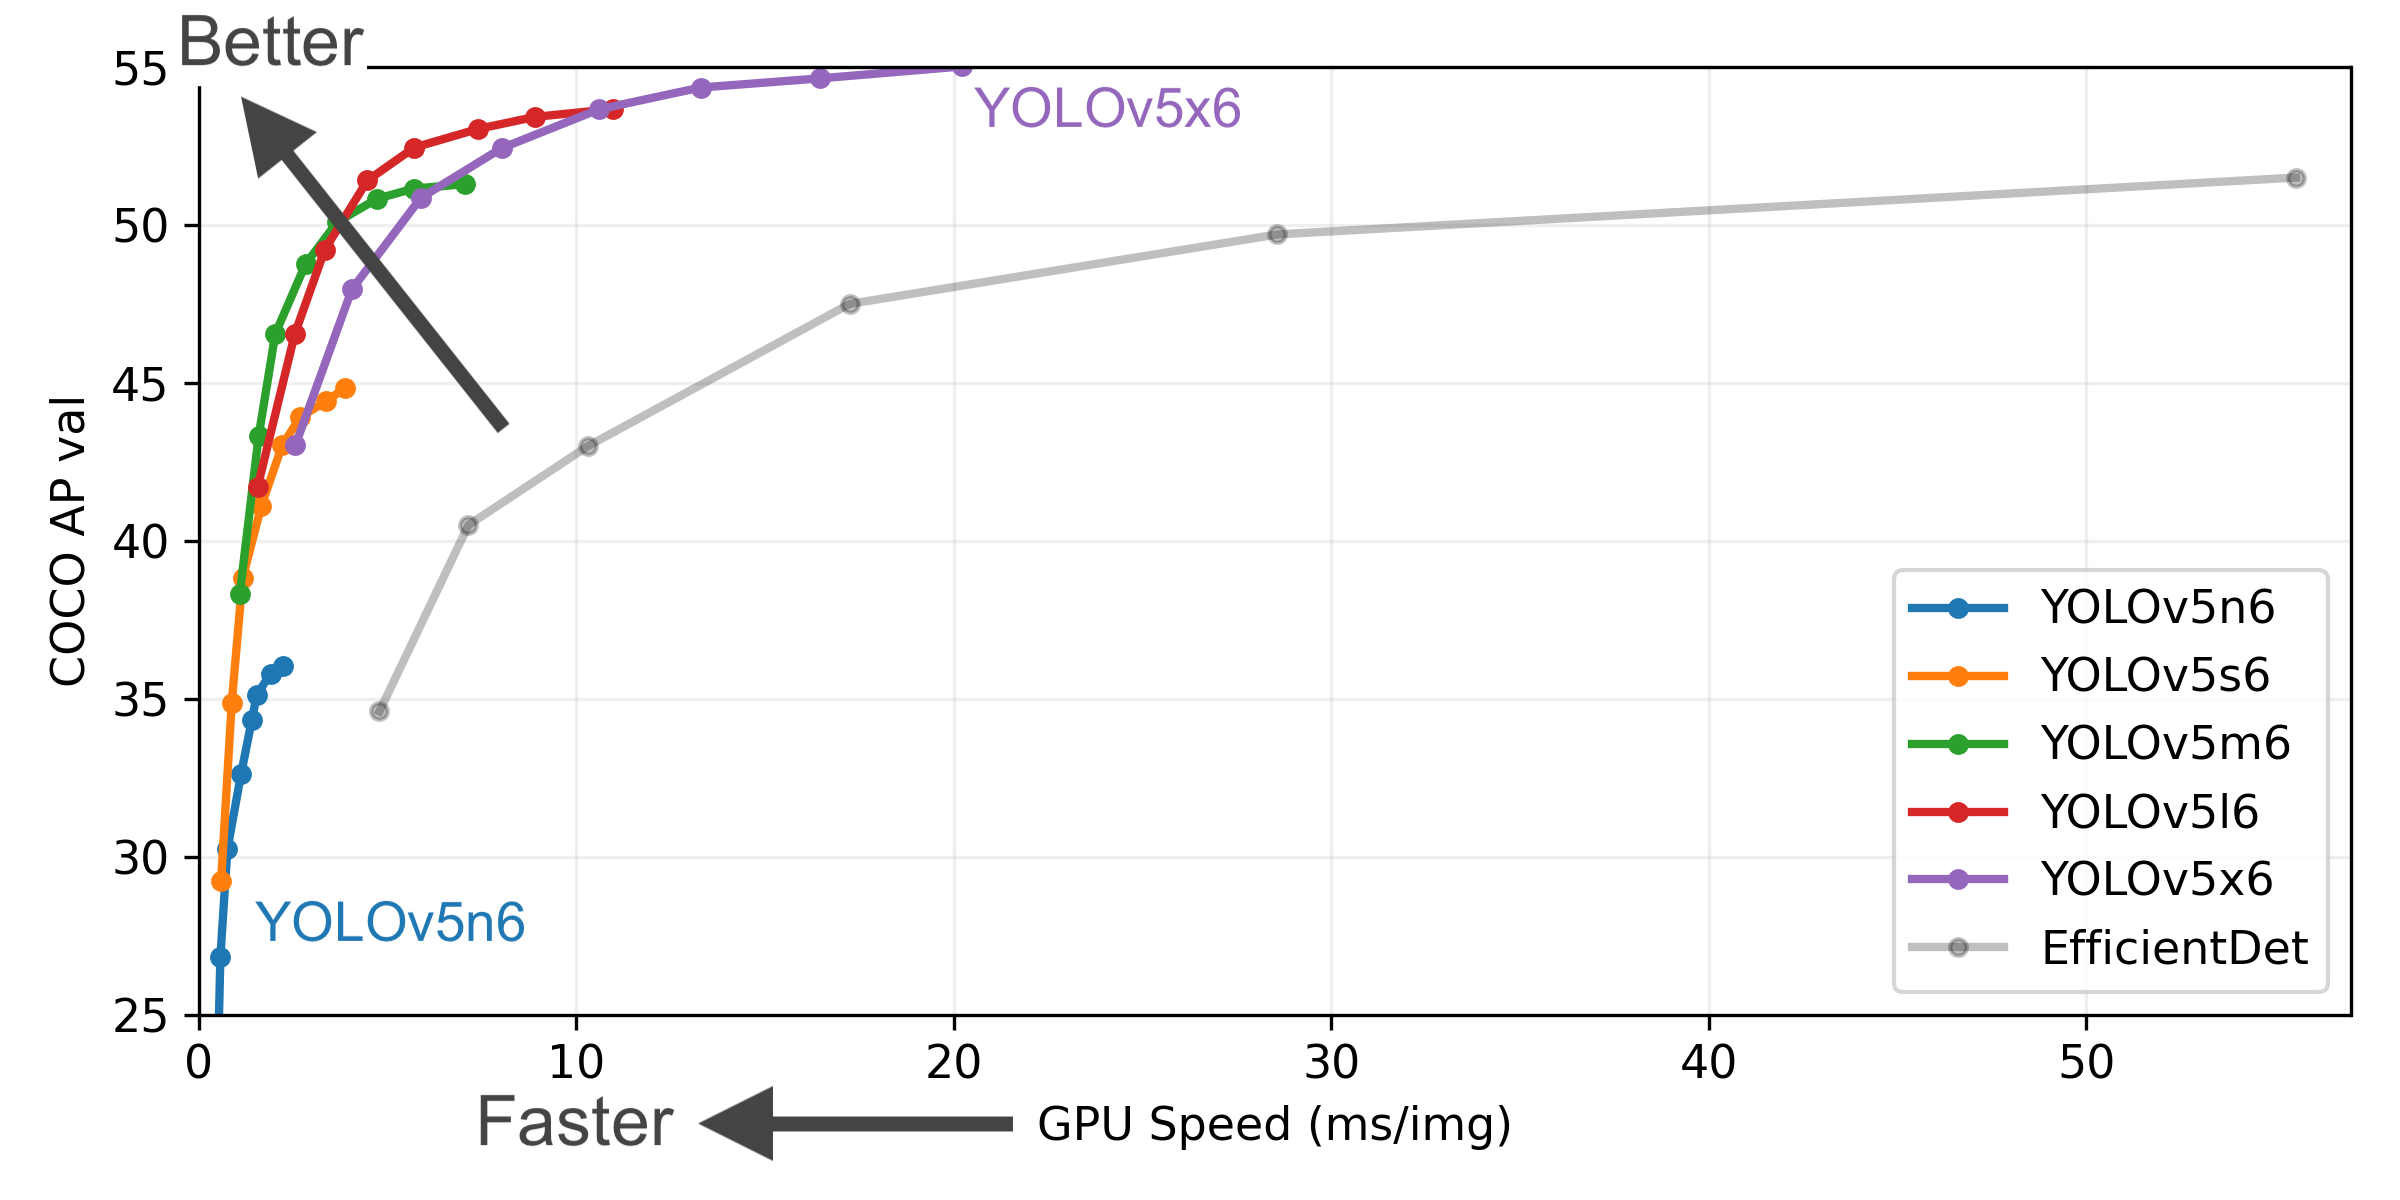
\includegraphics[width=\columnwidth]{images/yolov5-sizes.png}
    \end{center}

	\caption{Performance and speed comparison for the YOLOv5-v6.0 family of models considering the mAP@0.5:0.95 metric measured on the 5000-image COCO val2017 \cite{lin2014microsoft} dataset. The plot shows the performance of different models varying the input size of the image from $256 \times 256$px to $1536 \times 1536$px \cite{glenn_jocher_2021_5563715}.}
	\label{fig:yolo-sizes}%
\end{figure}


\begin{table}
    \centering
    \centerline{\begin{tabular}{c|c|c|c|c|c|c|c}
        \hline
        \multirow{2}{*}{ \textbf{Model}} & 
        \textbf{size} &
        \textbf{$\text{mAP}^{\text{val}}$} & 
        \textbf{$\text{mAP}^{\text{val}}$} & 
        \textbf{Speed} & 
        \textbf{Speed} & 
        \textbf{\# params} & 
        \textbf{FLOPs} \\
        & (pixels) & \textbf{0.5:0.95} & \textbf{0.5} & \textbf{CPU} (ms) & \textbf{GPU} (ms) & (M) & @640px (B) \\
        \hline
        YOLOv5n & 640 & 28.0 & 45.7 & 45 & 6.3 & 1.9 & 4.5 \\
        YOLOv5s & 640 & 37.4 & 56.8 & 98 & 6.4 & 7.2 & 16.5 \\
        YOLOv5m & 640 & 45.4 & 64.1 & 224 & 8.2 &  21.2 & 49.0 \\
        YOLOv5l & 640 & 49.0 & 67.3 & 430 & 10.1 & 46.5 & 109.1 \\
        YOLOv5x & 640 & 50.7 & 68.9 & 766 & 12.1 & 86.7 & 205.7 \\
        \hline
        YOLOv5n6 & 1280 & 36.0 & 54.4 & 153 & 8.1 & 3.2 & 4.6 \\
        YOLOv5s6 & 1280 & 44.8 & 63.7 & 385 & 8.2 & 12.6 & 16.8 \\
        YOLOv5m6 & 1280 & 51.3 & 69.3 & 887 & 11.1 &  35.7 & 50.0 \\
        YOLOv5l6 & 1280 & 53.7 & 71.3 & 1784 & 15.8 & 76.8 & 111.4 \\
        YOLOv5x6 & 1280 & 55.0 & 72.7 & 3136 & 26.2 & 140.7 & 209.8 \\
        \hline        
        \end{tabular}}
    \caption{Performance comparison considering the mAP@0.5:0.95 metric of all checkpoints of YOLOv5-v6.0 trained for 300 epochs on COCO dataset \cite{glenn_jocher_2021_5563715}.}
    \label{table:yolo-sizes}
\end{table}

The class-agnostic logo detector is based on YOLOv5m6, shown in \autoref{table:yolo-sizes}, with image input size set to $512 \times 512$px and pretrained on the COCO dataset. The model is then finetuned for 30 epochs on the task of class-agnostic logo recognition, thus, not distinguishing the specific logo class. 

\section{Classification}
\label{sec:method-classifier}
Given the ROIs, the classification of each cropped region is performed by a model trained using CIL techniques. To achieve this goal, the classifier is trained using the DER algorithm \cite{yan2021dynamically} described in \autoref{sec:der-algorithm}.

\subsection{ResNet-34}
\label{sec:resnet}
The DER algorithm introduces a new feature extractor $\mathcal{F}_t$ at each incremental step. This feature extractor consists of a Convolutional Neural Network (CNN). In the developed system, the backbone of the CNN used as feature extractor is ResNet-34 \cite{he2016deep} pre-trained on ImageNet1000 \cite{deng2009imagenet}.

The peculiar aspect of the ResNet architecture are the Residual Connections, shown in \autoref{fig:residual-connection}. These connections are a type of skip-connection that, instead of learning unreferenced functions, learn residual functions with respect to the layer inputs. Formally, denoting the desired underlying mapping as $\mathcal{H}(x)$, we let the stacked nonlinear layers fit another mapping of $\mathcal{F}(x) := \mathcal{H}(x) - x$. The original mapping is recast into $\mathcal{F}(x) + x$. 

The intuition is that it is easier to optimize the residual mapping than to optimize the original, unreferenced mapping. To the extreme, if an identity mapping were optimal, it would be easier to push the residual to zero than to fit an identity mapping by a stack of nonlinear layers \cite{he2016deep}.

The architecture of ResNet-34, shown in \autoref{table:resnet}, consists in multiple stacked building blocks. Each building block, represented by the brackets in \autoref{table:resnet}, adopt the residual connection described above.
The combination of both the skip-connection and the batch-normalization (BN) \cite{ioffe2015batch} in ResNet enable the training of an very deep neural network achieving high performance.
The total number of parameters of ResNet-34 used as feature extractor at each incremental step is 23 million.

\begin{table}
    \centering
    \begingroup
    
    \begin{tabular}{>{\centering\arraybackslash}p{.3\textwidth}|>{\centering\arraybackslash}p{.3\textwidth}|>{\centering\arraybackslash}p{.3\textwidth}}


        \hline
        \multicolumn{3}{c}{\textbf{ResNet-34 architecture}}\\
        \hline
        \textbf{Layer name} & \textbf{Output size} & \textbf{Layer} \\
        \hline
        \hline
        conv1 & $112 \times 122$ & $7 \times 7, 64,$ stride $2$ \\
        \hline
          & $56 \times 56$ & $3 \times 3$ max pool, stride $2$ \\
        \hline

        \[ \textrm{conv2\char`_x} \] &  \[56 \times 56 \] & \[\left[ \begin{array}{c} 3 \times 3, \, 64\\ 3 \times 3, \, 64  \end{array}\right] \times 3 \]\\
        \hline

        \[ \textrm{conv3\char`_x} \] &  \[28 \times 28 \] & \[\left[ \begin{array}{c} 3 \times 3, \, 128\\ 3 \times 3, \, 128  \end{array}\right] \times 4 \]\\
        \hline

        \[ \textrm{conv4\char`_x} \] &  \[14 \times 14 \] & \[\left[ \begin{array}{c} 3 \times 3, \, 256\\ 3 \times 3, \, 256  \end{array}\right] \times 6 \]\\
        \hline

        \[ \textrm{conv5\char`_x} \] &  \[7 \times 7 \] & \[\left[ \begin{array}{c} 3 \times 3, \, 512\\ 3 \times 3, \, 512  \end{array}\right] \times 3 \]\\
        \hline
        & $1000 \times 1$ & average pool \\
        \hline
        FC & $1000 \times 1$ & $1000$-d FC layer, softmax \\
        \hline
        \end{tabular}
    \endgroup
    \caption{Architecture of ResNet-34, the brackets represent a stack of building blocks. }
    \label{table:resnet}
\end{table}

\begin{figure}%
	\centering
	\subfloat[\centering Residual learning: a building block]{{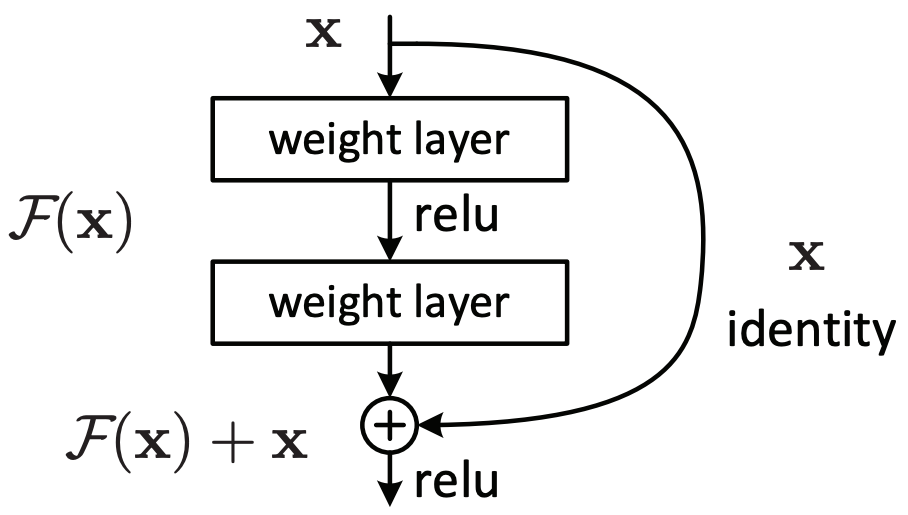
\includegraphics[width=0.45\textwidth]{images/residual-theory.png} }}%
	\hfill
	\subfloat[ An example of residual connection in a building block on a $56 \times 56$ feature maps. This building block corresponds to \textrm{conv2\char`_x} in \autoref{table:resnet} ]{{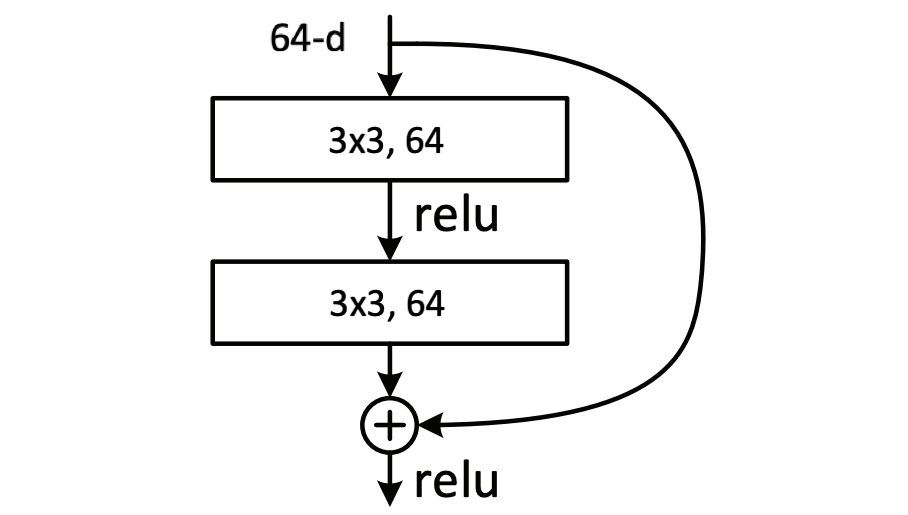
\includegraphics[width=0.45\textwidth]{images/residual-practice.png} }}%
	\caption{Residual connection in ResNet architecture \cite{he2016deep}.}%
	\label{fig:residual-connection}%
\end{figure}

\subsection{CIL classifier}
The classifier is developed in a CIL setup. In this way it is possible to recognize new logos by enriching the old knowledge. The algorithm used for CIL is the DER algorithm described in \autoref{sec:der-algorithm}. An implementation of the DER algorithm is given by PyCIL\footnote{PyCIL GitHub repository: \href{https://github.com/G-U-N/PyCIL}{https://github.com/G-U-N/PyCIL}}, and has been used as the starting for the development of the CIL classifier. All the changes performed to the implementation of DER in PyCIL are described in the following sections, and can be found in this\footnote{GitHub repository relative to the CIL model of this thesis: \\ \href{https://github.com/gianlucagiudice/PyCIL}{https://github.com/gianlucagiudice/PyCIL}} GitHub repository.


The implementation of DER in PyCIL reflects the description of the DER paper, the only change is relative to the third stage of the DER algorithm referred to as "Classifier Learning Stage" in \autoref{sec:der-algorithm}. In fact, in PyCIL the Classifier Learning Stage is performed using the WA described in \autoref{sec:wa-biased}; in this way it is possible to solve the problem of biased weights in the FC layer without the need to train the model further. It is important to point out that although this step of the original algorithm has been changed, the final performance reported by PyCIL is very similar to that obtained from the original DER paper (see \autoref{table:cil-results}).

\subsection{Regularization techniques}
In order to prevent overfitting of the model on the test set images, the architecture of the Neural Network (NN) created using the DER algorithm has been changed. Starting from the original architecture shown in \autoref{fig:der-pipeline}, a dropout layer has been added before the FC layer represented in the figure by the classifier $\mathcal{H}_t$.

\subsubsection{Dropout}
DNN with a large number of parameters are prone to overfitting the training data and do not generalize well on the test set.
Dropout \cite{srivastava2014dropout} is a technique for addressing this problem.

At training time, the units of the NN, along with their connections, are randomly dropped with a specified probability $p$ (a common value is $p = 0.5$). At test time, all units are present, but with weights scaled by $p$ (i.e. $w$ becomes $pw$). This procedure is shown in \autoref{fig:dropout}.

The idea is to prevent co-adaptation, where the NN becomes too reliant on particular connections, as this could be symptomatic of overfitting. Intuitively, dropout can be thought of as creating an implicit ensemble of NN.

\begin{figure}%
	\centering
	\subfloat[\centering Standard neural network]{{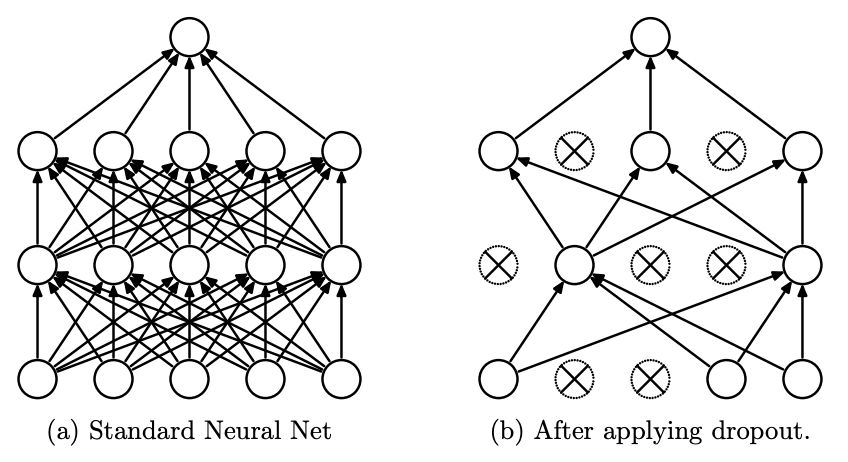
\includegraphics[width=0.30\textwidth,trim={0 24 220 0},clip]{images/dropout.png} }}%
	\hspace*{2cm}
	\subfloat[\centering Neural network after applying dropout ]{{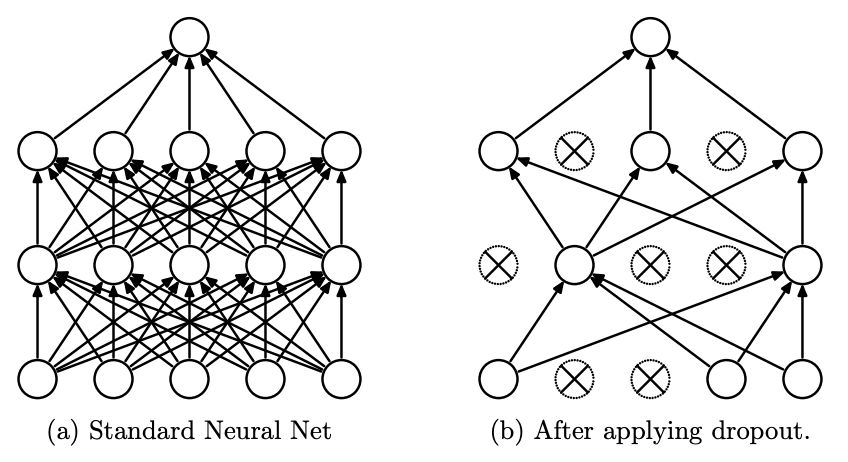
\includegraphics[width=0.30\textwidth,trim={220 24 0 0},clip]{images/dropout.png} }}%
	\caption{Dropout mechanism in a Neural Network with 2 hidden layers \cite{srivastava2014dropout}.}%
	\label{fig:dropout}%
\end{figure}

\subsection{Data Augmentation}
As discussed in \autoref{sec:dataset-stat}, one problem with the LogoDet-3K dataset is that some classes have a low number of images. Moreover, as shown in \autoref{table:logodet3k-quartile}, these classes are not the exception, but the majority of the classes in the dataset. In fact, the 50\% of the dataset has a number of images less than or equal to 54.

Training a model using a small number of examples per class can be a problem in machine learning in general, but this is especially true in the deep learning domain, where the models require a huge amount of data.

Image Augmentation is a data augmentation method that generates more training data from the existing training samples. This is a very useful technique to address the problem of the low number of images per class in LogoDet-3K. In addition, data augmentation is another helpful technique to avoid overfitting, as it creates synthetic samples by adding random elements the original image while preserving the main characteristics, thus achieve better generalization.

The type of data augmentation adopted during the training of the model is called online data augmentation. This technique consists in applying a random transformation to the original image before pass it to the model. In this way it is possible to achieve, in theory, an infinitely large dataset. The process of data augmentation is highly dependent on the type of transformations applied to the images: excessive transformation of the original image can mislead the model in learning the main features of the image, while keeping the image as similar as possible to the original image can have the same effect as not applying data augmentation at all.

Data augmentation is used for the training of the CIL classifier developed in this thesis. The transformations used to augment the original dataset, shown in \autoref{fig:example-augmentation}, are the following:
\begin{itemize}
    \item \textbf{Geometric transformations}:
    \begin{itemize}
        \item \textbf{Random affine}: transform the image keeping center invariant.
        \item \textbf{Random perspective}: perspective transformation of the image.
    \end{itemize}
    \item \textbf{Color transformations}:
    \begin{itemize}
        \item \textbf{Adjust sharpness}: adjusts the sharpness of the image by a sharpness factor.
        \item \textbf{Posterize}: reduces the number of bits for each color channel.
        \item \textbf{Color jitter}: randomly changes the brightness, contrast, saturation and hue of an image.
    \end{itemize}
\end{itemize}

As said before, the data augmentation is performed in an online manner, in this way it is possible to obtain slightly different image at each training epoch of the model. The original image is transformed using the transformations listed above, but the final transformed image is given by a combination of both geometric and color transformation. The procedure used to transform the original image is shown in \autoref{fig:data_augmentation}.


\begin{figure}%
	\centering

    \begin{center}
        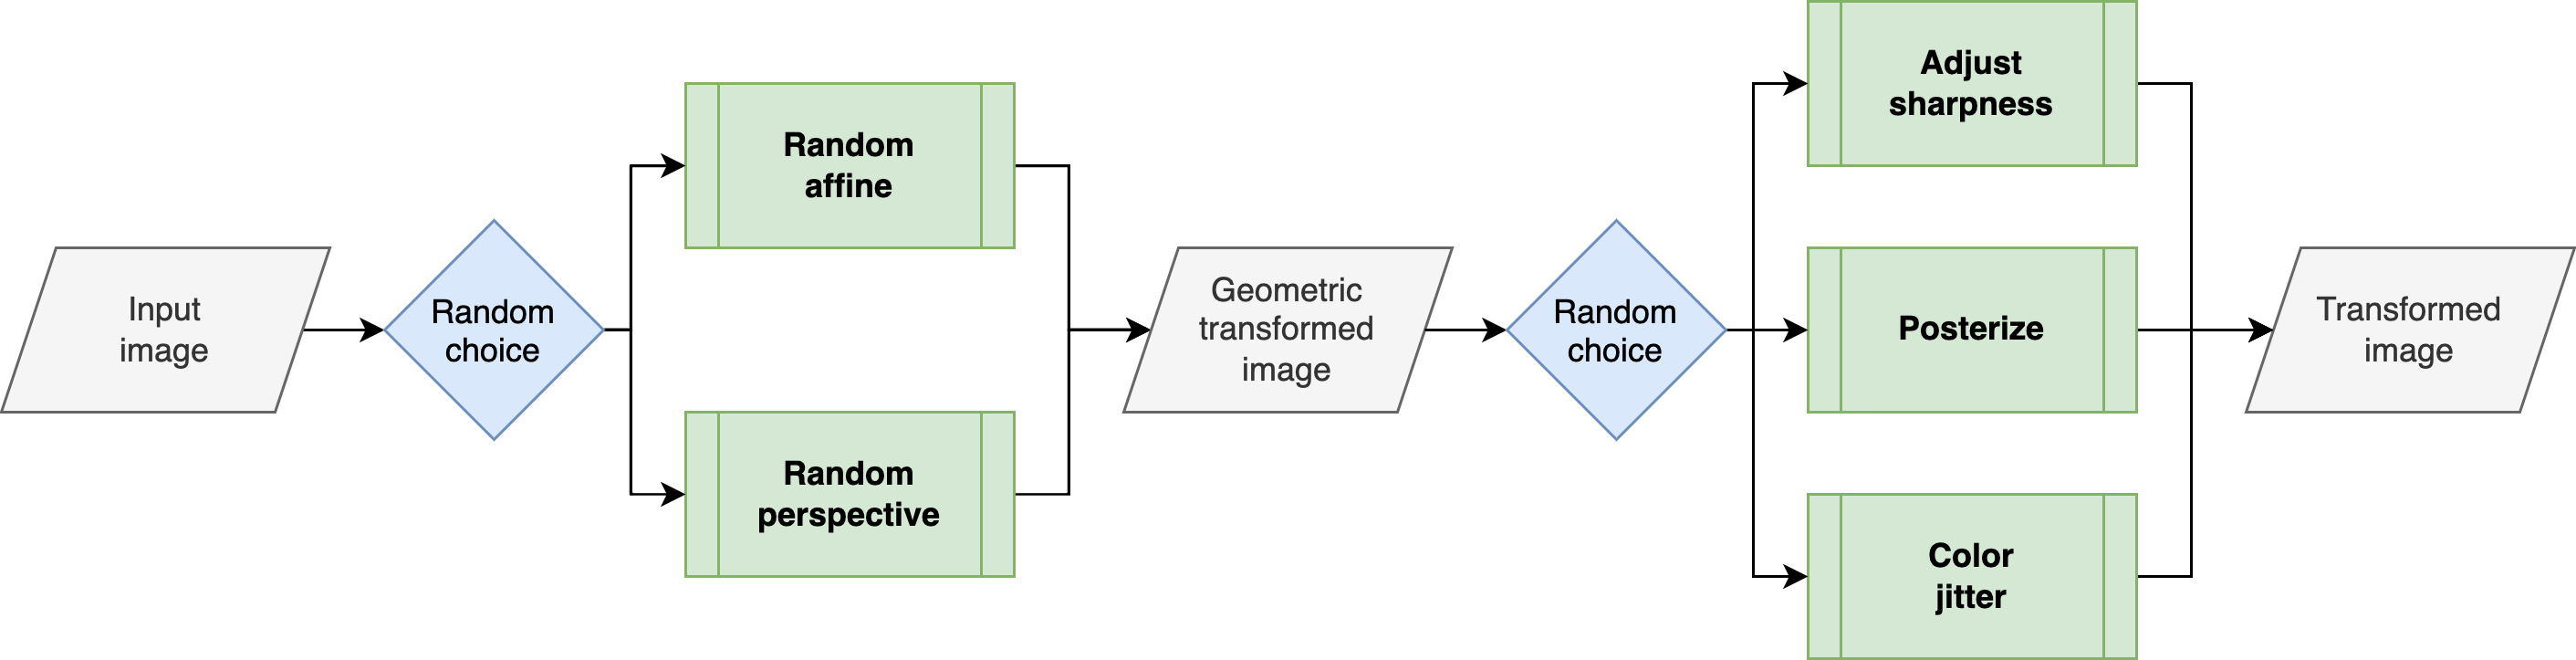
\includegraphics[width=\columnwidth]{images/data_augmentation.drawio.png}
    \end{center}

	\caption{Image transformation pipeline for data augmentation: first the input image is transformed via a geometric transformation, then a color transformation is applied.}%
	\label{fig:data_augmentation}%
\end{figure}

\begin{figure}%
	\centering
	\subfloat[Original image]{{
\includegraphics[height=3cm]{images/augmentations/original.jpg} }}%
	\hfill
	\subfloat[Random affine transformation]{{
\includegraphics[height=3cm]{images/augmentations/affine.jpg} }}%
	\hfill
	\subfloat[Random perspective transformation]{{
\includegraphics[height=3cm]{images/augmentations/perspective.jpg} }}%
	\hfill
	\subfloat[Adjust sharpness]{{
\includegraphics[height=3cm]{images/augmentations/sharpness.jpg} }}%
	\hspace*   {2cm}
	\subfloat[Posterize]{{
\includegraphics[height=3cm]{images/augmentations/posterize.jpg} }}%
	\hfill
    \subfloat[Random color Jitter]{{
\includegraphics[height=3cm]{images/augmentations/color_jitter.jpg} }}%
	\caption{Examples of image transformations. The transformations (d) and (e) are shown in a single image since, given the sharpness factor and the number of bin for the posterization, the result of the transformation is always the same.}%
	\label{fig:example-augmentation}%
\end{figure}

The data augmentation procedure, described in \autoref{fig:data_augmentation}, is applied to different logos in \autoref{fig:final_data_augmentation}.

\begin{figure}%
	\centering
	\subfloat[Logo 1]{{
\includegraphics[height=2cm]{images/augmentations/transf1.png} }}%
	\hfill
	\subfloat[Logo 2]{{
\includegraphics[height=2cm]{images/augmentations/transf2.png} }}%
	\hfill
	\subfloat[Logo 3]{{
\includegraphics[height=2cm]{images/augmentations/transf3.png} }}%
	\hfill
	\subfloat[Logo 4]{{
\includegraphics[height=2cm]{images/augmentations/transf4.png} }}%
	\hfill
    \subfloat[Logo 5]{{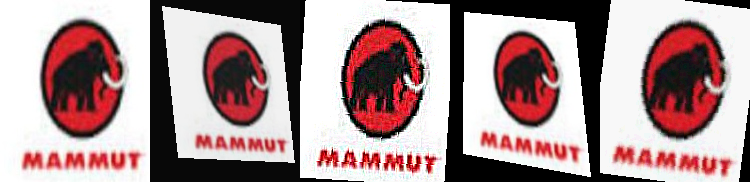
\includegraphics[height=2cm]{images/augmentations/transf5.png} }}%
	\hfill
    \subfloat[Logo 6]{{
\includegraphics[height=2cm]{images/augmentations/transf6.png} }}%
	\caption{Examples of data augmentation on different logos: the first column represents the original image, the other columns are some transformation applied to the original image following the pipeline described in \autoref{fig:data_augmentation}.}%
	\label{fig:final_data_augmentation}%
\end{figure}

\subsection{Training}
The training of the CIL model can be divided into two main steps: the initial step and the iterations of CIL. In the initial step the model is trained for 200 epochs, while for the incremental learning iterations it is trained for 150 epochs. 
This is done because, regarding the first step, the neural network has to adapt the weights trained on ImageNet to the logo classification task. We also assume that the number of classes at the initial task is greater than the number of classes that are introduced at each incremental learning iteration.


\subsubsection{Early stopping}
Early stopping is used to avoid overfitting of the model. This is done by monitoring the accuracy of the model during training on the validation set. For what concerns the hyperparameters of  early stopping, the number of epochs with no improvement after which training will be stopped is set to 30 (i.e. patience), and the minimum change in the monitored accuracy to qualify as an improvement is set to 0.5\% (i.e. minimum delta).

\subsubsection{SGD optimizer}
To update the model weights two different optimizers are tested. One of them is Stochastic Gradient Descent, an iterative method for optimizing an objective function.

As described in \cite{zhang2021dive}, in deep learning the objective function is usually the average of the loss functions for each example in the training dataset. Given a training dataset of $n$ examples, we assume that $f_i(\textbf{w})$ is the loss function with respect to the training example of index $i$, where $\textbf{w}$ is the parameter vector. Then the objective function is given by:
\begin{equation}
    f(\textbf{w}) = \frac{1}{n} \sum_{i=1}^n f_i(\textbf{w})
\end{equation}
The gradient of the objective function at $\textbf{w}$ is computed as:
\begin{equation}
    \nabla f(\textbf{w}) = \frac{1}{n} \sum_{i=1}^n \nabla f_i(\textbf{w})
\end{equation}
If gradient descent is used, the computational cost for each independent variable iteration is $\mathcal{O}(n)$, which grows linearly with $n$. Therefore, when the training dataset is larger, the cost of gradient descent for each iteration will be higher.

Stochastic gradient descent (SGD) reduces computational cost at each iteration. At each iteration of stochastic gradient descent, we uniformly sample an index $i \in \{ 1, \, ..., \, n\}$ for data examples at random, and compute the gradient $\nabla f_i (\textbf{w})$ to update $\textbf{w}$:

\begin{equation}
    \textbf{w} \leftarrow \textbf{w} - \eta \nabla f_i(\textbf{w})
\end{equation}
where $\eta$ is the learning rate ($\eta = 0.1$ in the experiments described in \autoref{chap:experiments}). In this way the computational cost for each iteration drops from $\mathcal{O}(n)$ of the gradient descent to the constant $\mathcal{O}(1)$. Moreover, the stochastic gradient $\nabla f_i(\textbf{w})$ is an unbiased estimate of the full gradient $\nabla f(\textbf{w})$ because:
\begin{equation}
    \mathbb{E}_i \nabla f_i(\mathbf{w}) = \frac{1}{n} \sum_{i = 1}^n \nabla f_i(\mathbf{w}) = \nabla f(\mathbf{w})
\end{equation}
This means that, on average, the stochastic gradient is a good estimate of the gradient.

A compromise between computing the true gradient and the gradient at a single sample is to compute the gradient against more than one training sample (called a "mini-batch") at each step. This means replacing the gradient $\nabla f_i(\textbf{w})$ on a single observation with one over a small batch $\mathcal{B}_t = \{ \textbf{x}^{(1)},\, ..., \, \textbf{x}^{(m)}\}$ (for the experiments described in \autoref{chap:experiments}, $|\mathcal{B}_t| = 2048$). Then, the gradient $\textbf{g}_t$ over a small batch $\mathcal{B}_t$ is given by:
\begin{equation}
    \mathbf{g}_t = \frac{1}{|\mathcal{B}_t|} \sum_{i \in \mathcal{B}_t} \nabla f_i(\mathbf{w})
\end{equation}
Note that, in an epoch, the examples are not reused for multiple batches. The minibatch SGD algorithm is shown in \autoref{alg:sgd} as described by Goodfellow et al. in \cite{Goodfellow-et-al-2016}.


\begin{algorithm}
    \caption{The Stochastic Gradient Descent (SGD) algorithm with minibatches}\label{alg:sgd}
    \begin{algorithmic}
        \Require Learning rate $\eta$
        \Require Initial parameters $\textbf{w}$
        
    \While{stopping criterion not met}
        
        Sample a minibatch $\mathcal{B}$ of $m$ examples from the training set $\{ \textbf{x}^{(1)},\, ..., \, \textbf{x}^{(m)}\}$ with corresponding labels $\textbf{y}^{(i)}$.

    Compute gradient estimate: $\hat{\mathbf{g}} = \frac{1}{|\mathcal{B}|} \sum_{i \in \mathcal{B}_t} \nabla f_i(\mathbf{w})$.

    Apply update: $\textbf{w} \leftarrow \textbf{w} - \eta \hat{\mathbf{g}}$.

    \EndWhile
    \end{algorithmic}
    \end{algorithm}


\subsubsection{Adam optimizer}
The second optimizer used in the experiments is Adam \cite{kingma2014adam}, which can be considered as a combination of RMSProp \cite{hinton2012neural} and momentum \cite{sutskever2013importance}. Adam is an adaptive learning rate optimizer, i.e. it uses a separate learning rate for each parameter and automatically adapt these learning rates throughout the course of learning. A key component of Adam is that it uses exponential weighted moving averages (also known as leaky averaging) to obtain an estimate of both the momentum and also the second moment of the gradient.

To estimate the first-order and the second-order moments of the gradient, Adam uses two state variables:
\begin{equation}
    \begin{split}\begin{aligned}
        \mathbf{v}_t & \leftarrow \beta_1 \mathbf{v}_{t-1} + (1 - \beta_1) \mathbf{g}_t \\
        \mathbf{s}_t & \leftarrow \beta_2 \mathbf{s}_{t-1} + (1 - \beta_2) \mathbf{g}_t^2
    \end{aligned}\end{split}
\end{equation}
where $\beta_1$ and $\beta_2$ are nonnegative weighting parameters. In the experiments in \autoref{chap:experiments}, $\beta_1=0.9$ and $\beta_2=0.999$.

Initially, both $\mathbf{v}_0$ and $\mathbf{s}_0$ are set to 0, resulting in a bias towards smaller values. For this reason, Adam computes the bias-corrected $\hat{\mathbf{v}}_t$ and $\hat{\mathbf{s}}_t$ as follows:
\begin{equation}
    \begin{split}\begin{aligned}
        \hat{\mathbf{v}}_t & = \frac{\mathbf{v}_t}{1 - \beta_1^t} \\
        \hat{\mathbf{s}}_t & = \frac{\mathbf{s}_t}{1 - \beta_2^t}
    \end{aligned}\end{split}
\end{equation}
Then, the gradient is rescaled accordingly to consider both the first-order and second-order moments:
\begin{equation}
    \mathbf{g}_t' = \eta \frac{ \hat{\mathbf{v}}_t}{\sqrt{\hat{\mathbf{s}}_t} + \epsilon}
\end{equation}
where, $\eta$ is the learning rate (set to $0.001$ in the experiments in \autoref{chap:experiments}) and $\epsilon = 10^{-8}$ is a constant to achieve numerical stability.

Finally, the parameters are updated as follows:
\begin{equation}
    \textbf{w}_t \leftarrow \textbf{w}_{t-1} - \mathbf{g}_t'
\end{equation}

The Adam algorithm is shown in \autoref{alg:adam} as described by Goodfellow et al. in \cite{Goodfellow-et-al-2016}.

\begin{algorithm}
    \caption{The Adam algorithm}\label{alg:adam}
    \begin{algorithmic}
        \Require Learning rate $\eta$
        \Require Exponential decay rates for moment estimates, $\beta_1$ and $\beta_2$ in $[0, \, 1)$ (Suggested defaults: $0.9$ and $0.999$ respectively).
        \Require Small constant $\epsilon$ used for numerical stabilization (Suggested default: $10^{-8}$).
        \Require Initial parameters $\textbf{w}$\\
        Initialize 1st and 2nd moment variable $\mathbf{s} = 0$, $\mathbf{r} = 0$\\
        Initialize time step $t = 0$
    \While{stopping criterion not met}
        
        Sample a minibatch $\mathcal{B}$ of $m$ examples from the training set $\{ \textbf{x}^{(1)},\, ..., \, \textbf{x}^{(m)}\}$ with corresponding labels $\textbf{y}^{(i)}$.
        
        Compute gradient estimate: $\hat{\mathbf{g}} = \frac{1}{|\mathcal{B}|} \sum_{i \in \mathcal{B}_t} \nabla f_i(\mathbf{w})$.

        $t \leftarrow t +1$
        
        Update biased first moment estimate: $\mathbf{v} \leftarrow \beta_1 \mathbf{v} + (1 - \beta_1) \mathbf{\hat{g}}$

        Update biased second moment estimate: $\mathbf{s} \leftarrow \beta_2 \mathbf{s} + (1 - \beta_2) \mathbf{\hat{g}}^2$

        Correct bias in first moment: $\hat{\mathbf{v}} = \frac{\mathbf{v}}{1 - \beta_1^t}$
  
        Correct bias in second moment: $\hat{\mathbf{s}} = \frac{\mathbf{s}}{1 - \beta_2^t}$

        Compute update: $\Delta \mathbf{w} = \eta \frac{ \hat{\mathbf{v}}}{\sqrt{\hat{\mathbf{s}}} + \epsilon}$

        Apply update: $\textbf{w} \leftarrow \textbf{w} - \Delta \mathbf{w}$.

    \EndWhile
    \end{algorithmic}
    \end{algorithm}

\subsubsection{Learning rate decay}
For both the optimizers, an exponential decay scheduling is applied to the learning rate: once the number of epoch reaches one of the predetermined epochs, called milestones, the learning rate of the optimizer is multiplied by a factor $\gamma = 0.1$. The milestones are set to 60, 100 and 150 for the initial learning stage, and to 40, 75, 100 for each incremental learning iteration.

Adjusting the learning rate is an important aspect of the optimization process; some of the motivations behind learning rate scheduling are described below:
\begin{itemize}
    \item The magnitude of the learning rate is a key factor in the optimization procedure: if the learning rate is too large, optimization diverges, while if it is too small, either training takes too long or a suboptimal result is achieved.
    \item If the learning rate remains high, the algorithm may bounce around the minima or even jump over the minima and thus failing to reach optimality. 
\end{itemize}

The learning rate decay is used to train the models for the experiments described in \autoref{chap:experiments}. An example of the effect of the learning rate decay is shown in \autoref{fig:lr_decay}. The figure shows the accuracy of the model at each training epoch, it can be seen that when a milestone is reached (epoch 60) the learning rate is scaled by a fact of $10^{-1}$, thus leading to an increase in the model's accuracy in subsequent epochs.

\begin{figure}[H]
	\centering

    \begin{center}
        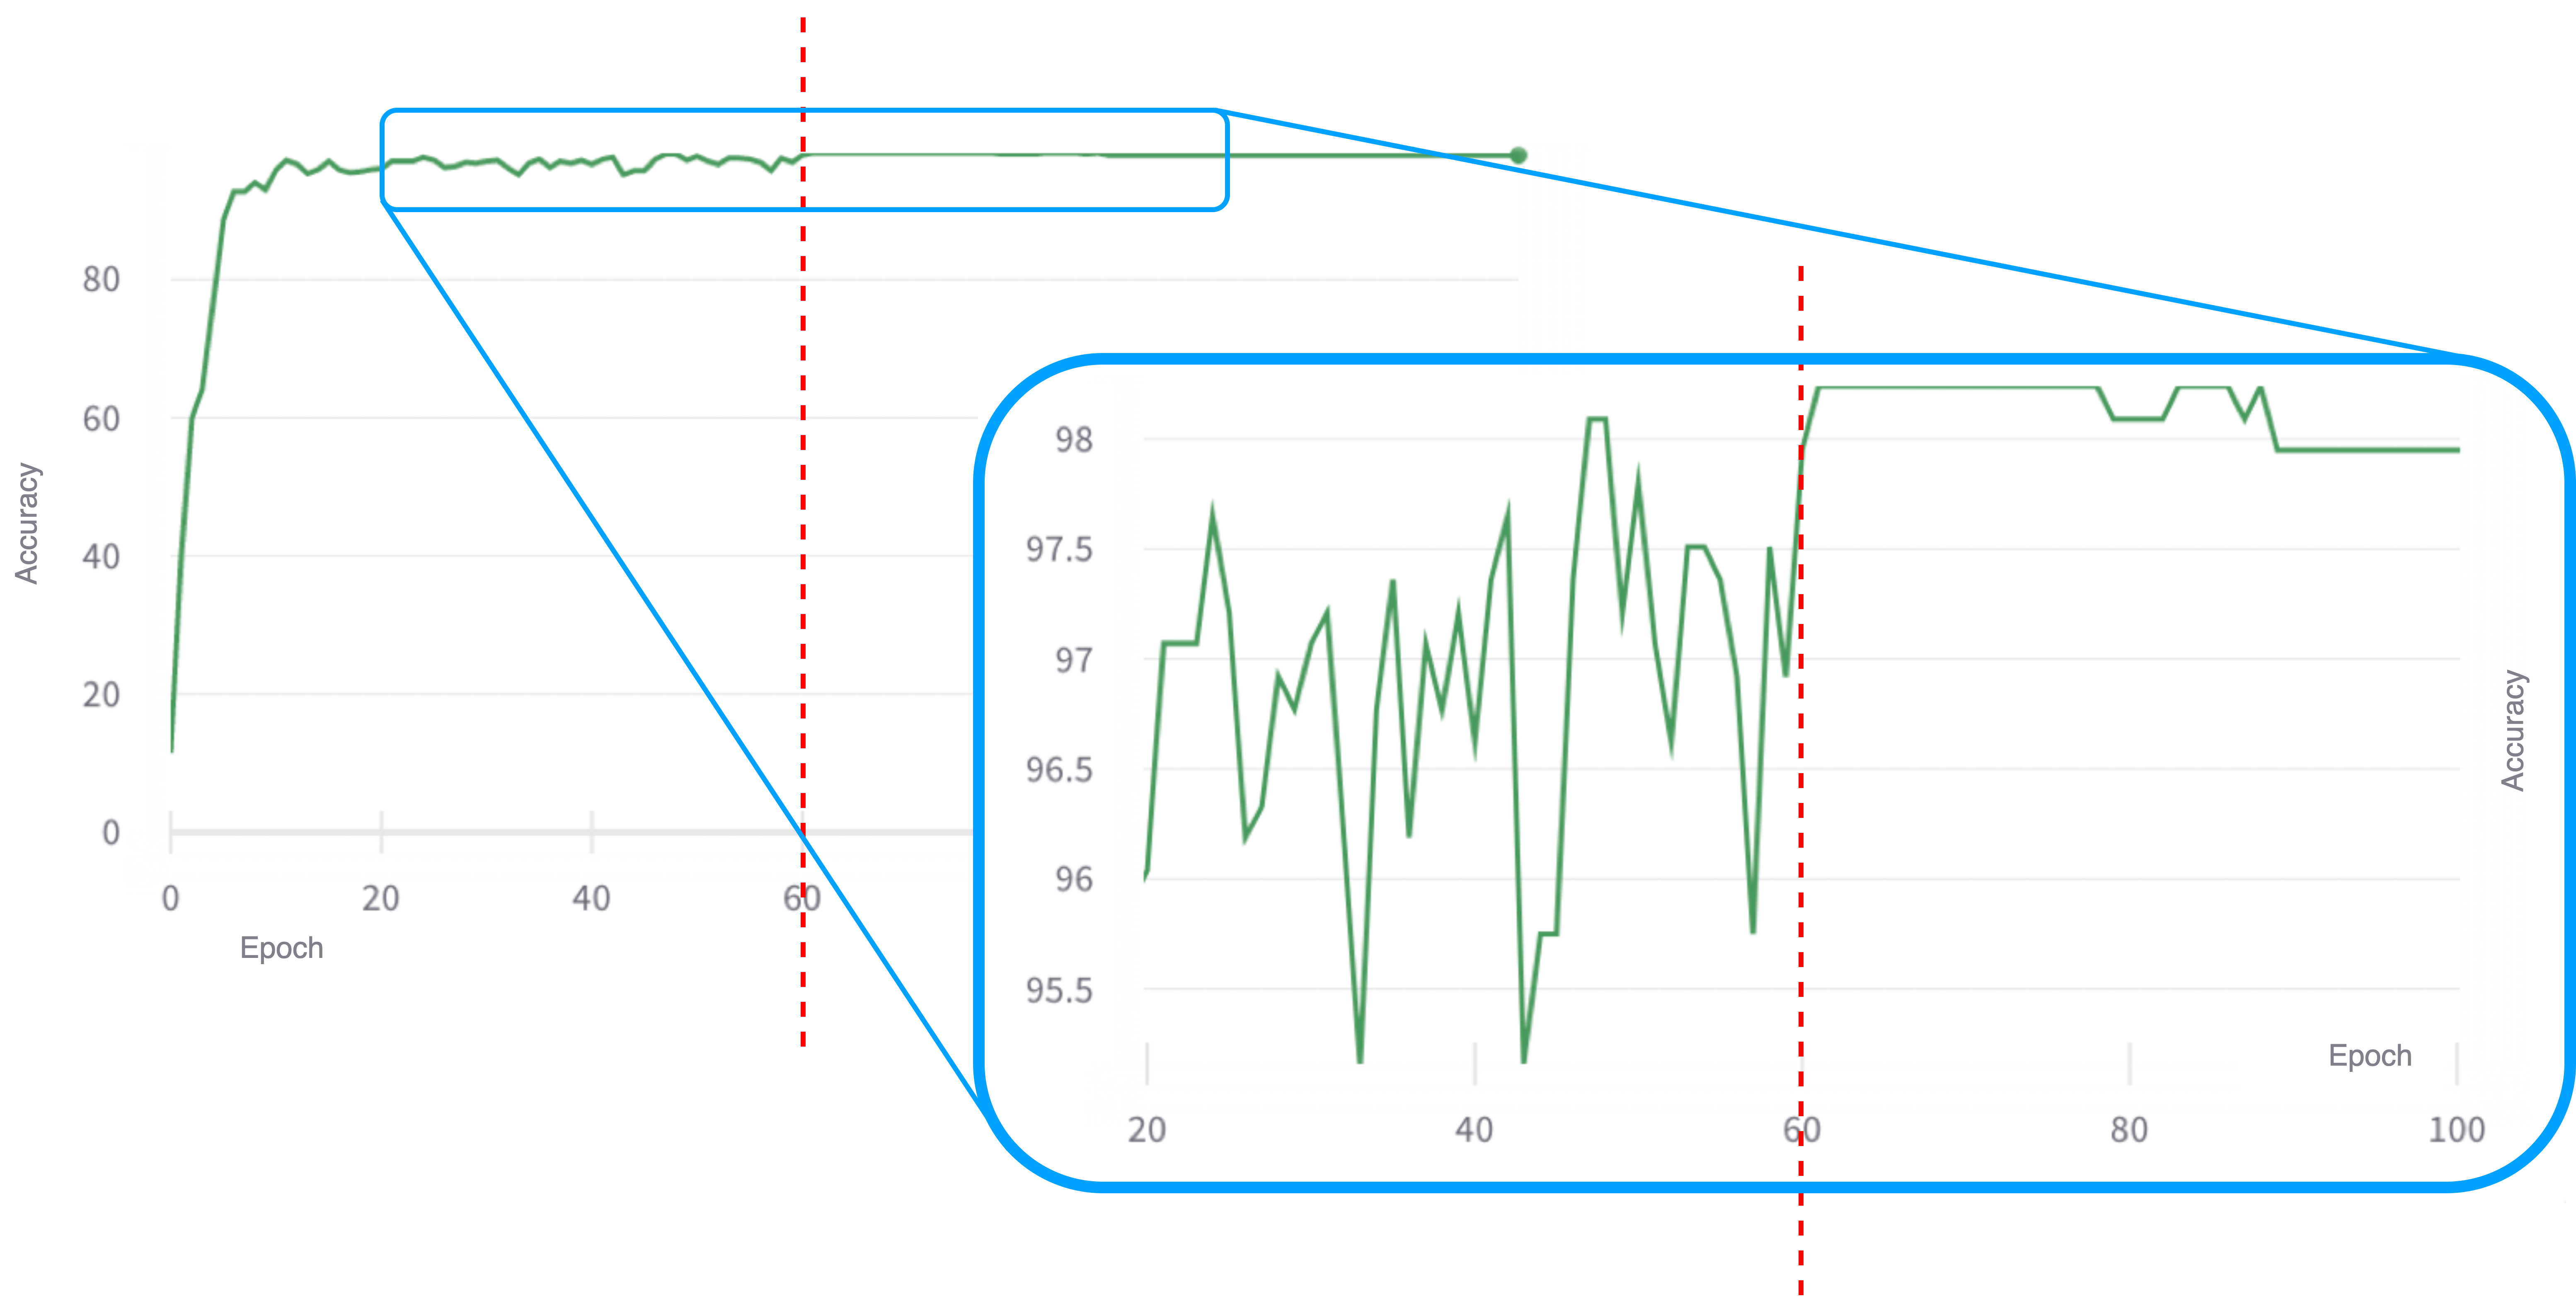
\includegraphics[width=\columnwidth]{images/lr_decay.drawio.png}
    \end{center}

	\caption{Effect of the learning rate decay: the figure shows the accuracy of the model at each training epoch. At epoch 60, the learning rate is scaled by a factor of $10^{-1}$, this leads to an increase in the model's accuracy in subsequent epochs. }
	\label{fig:lr_decay}%
\end{figure}


\subsection{Pruning}
\label{sec:method-pruning}

The DER algorithm, described in \autoref{sec:der-algorithm}, addresses the problem of class incremental learning by expanding the neural network architecture at each incremental stage. The super-feature extractor at step $t$ of incremental learning is given by the following concatenation $\Phi_t(\mathbf{x}) = [\mathcal{F}_0,\mathcal{F}_1(\mathbf{x}), \, ..., \, \mathcal{F}_t(\mathbf{x})]$. As discussed in \autoref{sec:resnet}, the feature extractors consists of a CNN that corresponds to ResNet-34 in the system implementation of this thesis.

Each feature extractor, i.e. ResNet-34, is a CNN with 22 million parameters. Giving the definition of the super-feature extractor, it is possible to see how the parameters how the neural network grow linearly as a function of the number of incremental learning stages. It is important to note that as the number of parameters of the super-feature extractor increases, the number of parameters for the classifier $\mathcal{H}_t$ also increases.
The classifier $\mathcal{H}_t$ corresponds to the fully connected layer of the neural network; at each incremental learning stage, new classes are introduced, thus new connections are created between the classifier predicting the output class and the super-feature extractor.

This means that, using the LogoDet-3K dataset described in \autoref{chap:dataset}, and the incremental learning setup described in \autoref{sec:whole_dataset_clf}, at the 8th stage of CIL the neural network consists of 205 million parameters. This number of parameters is due to task 0 (initial task), in which 22 million parameters are used, and the 8 incremental learning stages, each of which adds approximately 22 million parameters to the total number of parameters.

After only eight iterations of incremental learning, the final neural network reaches 205 million parameters, which is quite a high number of parameters. 
For this reason, there is a need to reduce the number of parameters of the neural network.
To do so, the pruning of the network is implemented using masks, as described in \autoref{sec:masking-pruning}.

Each mask $\mathbf{m}_l$ associated with the channels of each layer $l$ of the CNN is computed as shown in \autoref{eq:mask}.
At the incremental learning task $t$, after the training of the feature extractor $\mathcal{F}_t(\mathbf{x})$, the variable $s$ is set to a really high value ($10^{4}$ in the implementation). Since $s$ in fed into the sigmoid used as gating function, this results in a stepwise activation mechanism (this is true in the limit but is achieved in practice using high value of $s$). Then, if a value $e_{li}$ of the mask $\mathbf{e}_l$ is positive, $m_{li}$ tends to 1, whereas if $e_{li}$ is negative, $m_{li}$ tends to 0. Finally, to perform the actual binarization of each mask value, a threshold $\rho$ with a low value set to $10^{-4}$ is used as follows:


\begin{align*}
    m_{li}&=\left\{
        \begin{array}{@{}ll@{}}
            1, & \text{if } m_{li} > \rho\\
            0, & \text{if } m_{li} \leq \rho\\
        \end{array}\right.\\
\end{align*}

An important aspect to consider during the pruning of each convolutional layers $l$ of the feature extractor $\mathcal{F}_t(\mathbf{x})$ is the input and output dimension of the feature maps.
Since $\mathbf{m}_l$ is a channel-level mask, the effect of pruning is to reduce the number of channels in the convolutional layers of the CNN.
This results in altering the output dimension of the convolutional layer $l$, so the input dimension of the convolutional layer $l+1$ must be consistent with the output dimension of the tensor of the convolutional layer $l$.

Another point to consider is the architecture used to implement the feature extractors $\mathcal{F}_t$. In fact, each feature extractor has as its backbone ResNet-34, which is an architecture based on residual connections (see \autoref{table:resnet} and \autoref{fig:residual-connection}).
This is a limitation from a pruning perspective, because not only each feature map produced as output from a convolutional layer must have a dimension consistent with the input of the next convolutional layer, but there is the additional constraint caused by the residual connections that must also be consistent with the dimension of the input of the convolutional layers. This issue is shown and described in \autoref{fig:pruning-resnet}.


\begin{figure}[H]
    \begin{center}
        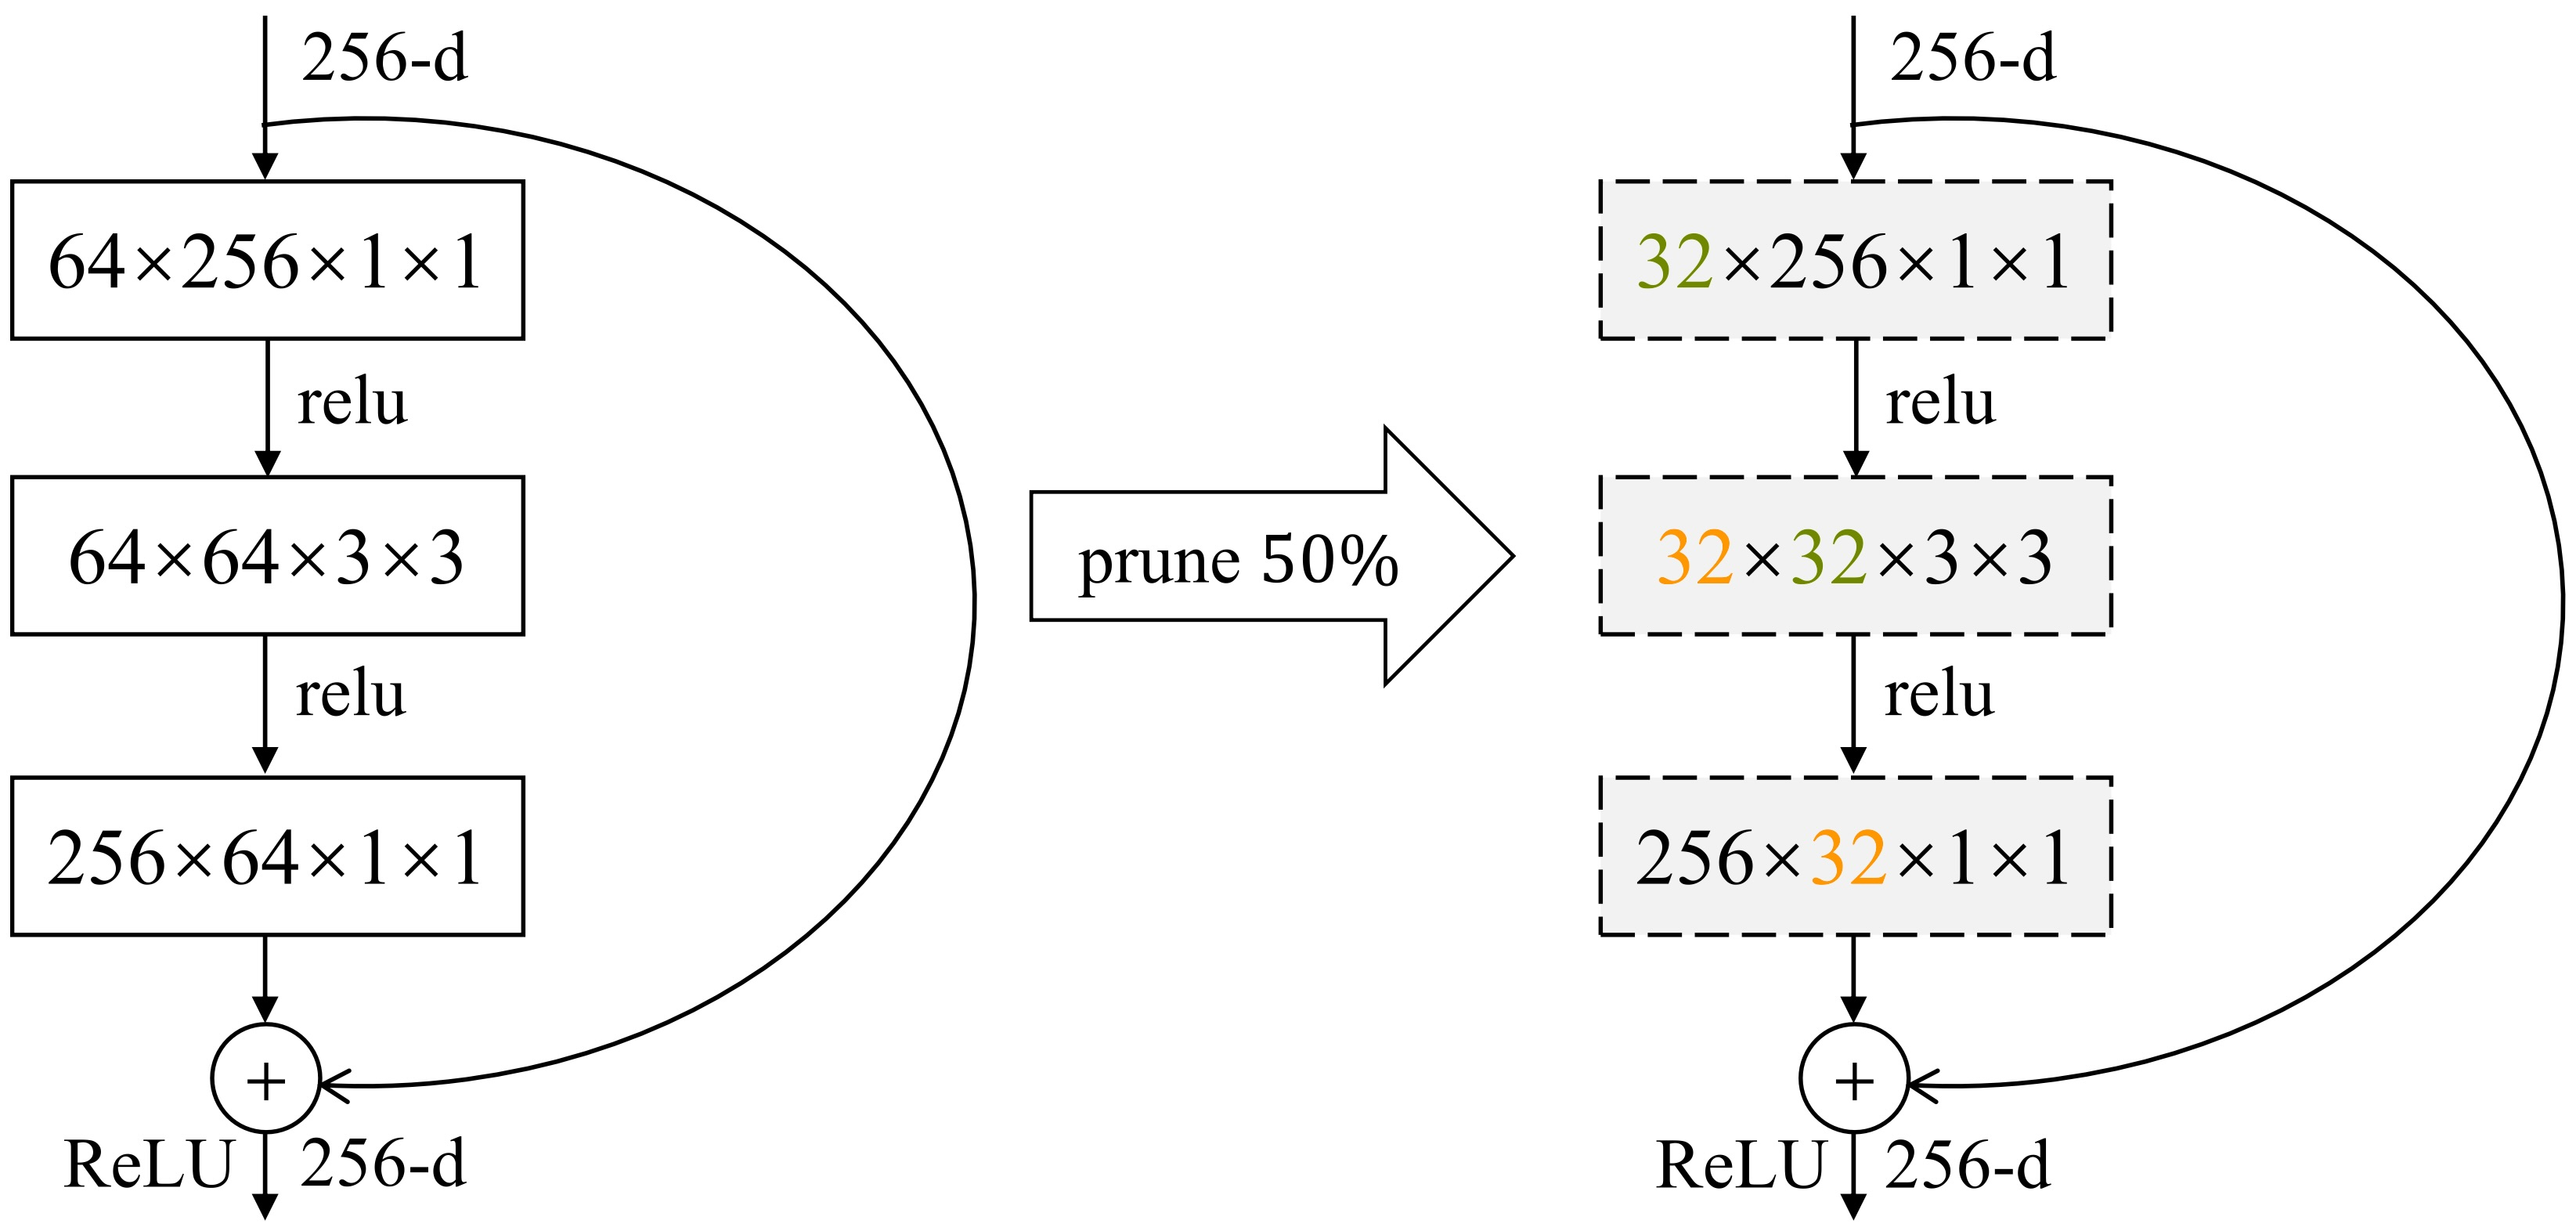
\includegraphics[width=\columnwidth]{images/resnet-pruning.png}
    \end{center}
    \caption{Pruning strategy of ResNet. The pruning is performed in such a way that the final size of the output is maintained, so that the residual connection can be added. Image from \cite{8416559}.}
    \label{fig:pruning-resnet}
\end{figure}

The use of residual connections involves pruning at block level.
The definition of block depends on the specific ResNet architecture, but in the case of ResNet-34, a block consists of two convolutional layers, as shown in \autoref{table:resnet}, so pruning is applied to pairs of convolutional layers.
This approach is necessary to maintain a feature maps in which the identity carried by the residual connection can be added.

\section{Knowledge distillation}
\label{sec:method-kd}

\begin{figure}[H]%
	\centering

    \begin{center}
        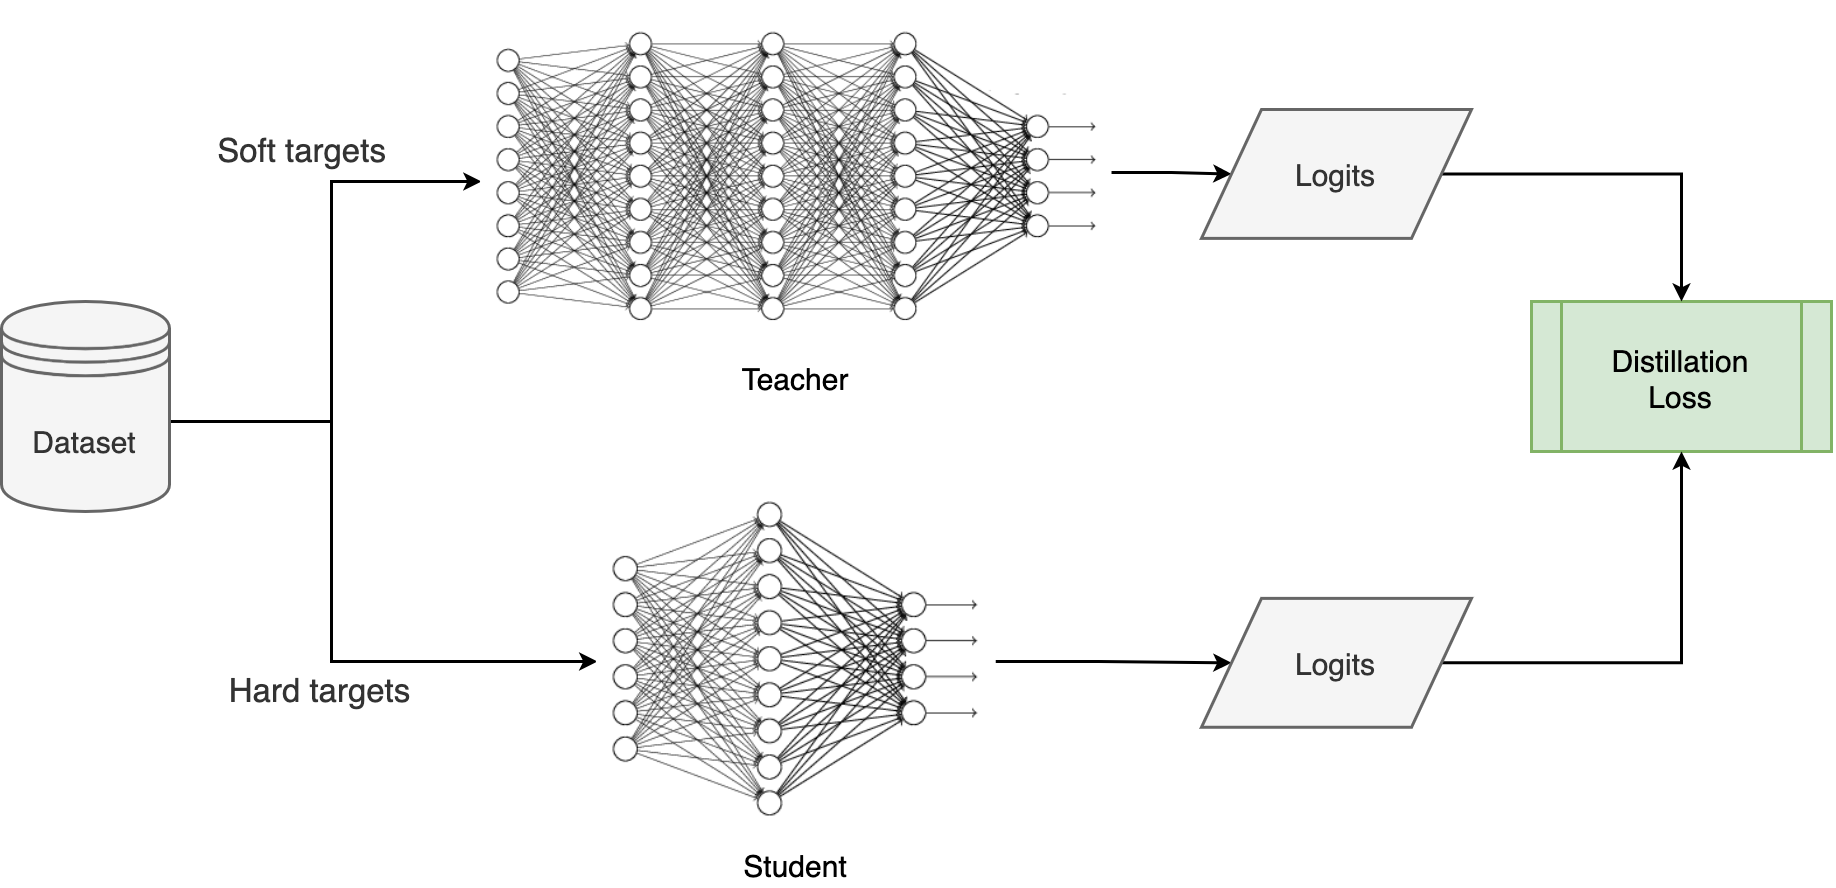
\includegraphics[width=\columnwidth]{images/kd.drawio.png}
    \end{center}

	\caption{Knowledge distillation pipeline: the student model is trained by exploiting the teacher model using the distillation loss. This loss considers both the logits of the teacher and the real data labels.}%
	\label{fig:kd}%
\end{figure}

Another approach used to address the problem of the large number of model parameters described in the previous section is Knowledge Distillation (KD) \cite{hinton2015distilling}. Knowledge distillation is the process of transferring knowledge from a large model to a smaller one. While large models (such as very deep neural networks like ResNet-152) have higher knowledge capacity than small models, this capacity might not be fully utilized.

KD is essentially a model compression method in which a small model is trained to mimic a pre-trained, larger model.
A large model with regularization (e.g. using dropout) generalizes better than a small model when trained directly on the data and labels, however, a small model can be trained to generalize better with help of a large model. This training setting is referred to as "teacher-student", where the large model is the teacher and the small model is the student.

As described by Gou et al. in \cite{gou2021knowledge},
Response-Based Knowledge is a type of KD which refers to the neural
response of the last output layer of the teacher model.
In thesis, the implementation of the KD is based on the paper of Hinton et al. in \cite{hinton2015distilling}.
The main idea is to directly mimic the final prediction
of the teacher model.
The reason behind this is that the output probabilities of a trained model give more information than the labels because it assigns non-zero probabilities to incorrect classes as well.
Knowledge is transferred from the teacher model to the student using a loss function known as the distillation loss, which captures the difference between the logits of the student and teacher models. In this way, the student become more accurate in making predictions similar to the teacher as this loss is reduced over time. The teacher-student setting for KD matching the logits between the two models is shown in \autoref{fig:kd}.

The distillation loss used to train the student model is computed considering both the logits produced in output by the teacher and the real data labels.
The probability $p_i$ of each class $i$, is computed by the teacher model using its logits $z_i$ as follows:
\begin{equation}
    p_i = \frac{exp(z_i)}{\sum_j exp(z_j)}
\end{equation}

The small model is trained to minimize the KL Divergence between its output probability distribution and the large network's output probability distribution (soft targets).

One issue with this technique is that the probabilities assigned to incorrect classes by the large network are often very small and don't contribute to the loss. For this reason, the logits are softened using a "temperature" $T$ in the softmax, effectively smoothing out the probability distribution and revealing inter-class relationships learned by the teacher. Then, the softened probabilities are given by:
\begin{equation}\label{eq:kd_prob}
    p_i^t = \frac{exp(\frac{z_i^t}{T})}{\sum_j exp(\frac{z_i^t}{T})}
\end{equation}
where higher values for $T$ will produce softer probabilities. The predictions $p_i^t$ are called soft targets, shown in \autoref{fig:kd}.

In the same way, the \autoref{eq:kd_prob} is used to compute the class probabilities $p_i^s$ predicted by the student using the logits $z_i^s$ of the model and the same temperature $T$. In addition to the teacher's soft targets, Hinton et al. in \cite{hinton2015distilling} show that it is also beneficial to train the student model to produce the real data labels, called hard targets and shown in \autoref{fig:kd}.
Therefore, by setting $T = 1$, the \autoref{eq:kd_prob} is used to compute the "standard" class probabilities $\hat{y}_i^s$ using the student model.

Thus, considering both the KL divergence of the output probability distribution of the two models, and the Cross-Entropy between the output probabilities $\hat{y}_i^s$ of the student and the true data labels $y_i$, the final distillation loss is given by:
\begin{equation}
    \mathcal{L}_{KD} = \alpha \left[\sum_{i=1}^{\substack{\text{output}\\\text{size}}} p_i^t \, log \left( \frac{p_i^t}{p_i^s} \right) \right]
    + (1-\alpha) \left[-\sum_{i=1}^{\substack{\text{output}\\\text{size}}} y_i^s \, (\log \hat{y}_i^s) \right]
\end{equation}
where $\alpha \in [0, 1]$ is a hyper-parameter controlling the weighted average between the two components.

\section{Proposed baseline for the classifier}
\label{sec:method-baseline}
To evaluate CIL models and compare performance with a model in a traditional setup, without the possibility of introducing new classes after training, there is a need to define a baseline. CIL models are very useful for introducing new classes after training, but in general this advantage is at the expense of model performance. Consequently, a CIL model will perform less well when compared to one trained in a traditional setup, but a good CIL algorithm should narrow this gap as much as possible. 

Since, without considering the CIL aspect, different approaches can be defined to handle a classical classification problem, this chapter discusses the different baselines introduced with the aim of comparing them with the CIL models.

\subsection{Baseline without incremental steps}
The most direct approach is to define a baseline using the DER algorithm. This means taking all the classes introduced incrementally at each iteration of incremental learning, and using them from the very beginning at task 0 to train the model with the DER algorithm. The foregoing defines the first type of baseline considered for comparison with the CIL model.

Although this approach appears to be simple and straightforward, it has a problem related to what is described in section \autoref{sec:method-pruning}. In fact, such an approach is not very fair, as the baseline has a number of parameters $N$ equal to the CNN used as the backbone for the feature extractor, whereas the CIL model trained with the DER algorithm will have a number of parameters equal to $N + t \times N$, where $t$ is the number of iterations of incremental learning. As a result, the CIL model may perform better than the baseline only because it has a significantly larger number of parameters.

\subsection{ResNet-152 architecture}
In order to solve the problem of the first baseline definition, relating to the difference in parameters between the baseline and the CIL model, a second type of baseline is defined. In this second approach, the DER algorithm is not used anymore but simply a network with a significantly higher number of parameters, e.g. ResNet-152, is used in order to bridge the gap in the number of parameters between the baseline and the CIL model.

A CNN that has ResNet-152 as a backbone is then used. The architecture of ResNet-152 is very similar to the one described in the table \autoref{table:resnet}, in fact it maintains all the main features such as skip-connections, but has each block composed of more convolutional layers, and the number of stacked blocks increases. The architecture of ResNet-152 consists of 60 million parameters and is described in \autoref{table:resnet-152}.


\begin{table}
    \centering
    \begingroup
    
    \begin{tabular}{>{\centering\arraybackslash}p{.3\textwidth}|>{\centering\arraybackslash}p{.3\textwidth}|>{\centering\arraybackslash}p{.3\textwidth}}


        \hline
        \multicolumn{3}{c}{\textbf{ResNet-152 architecture}}\\
        \hline
        \textbf{Layer name} & \textbf{Output size} & \textbf{Layer} \\
        \hline
        \hline
        conv1 & $112 \times 122$ & $7 \times 7, 64,$ stride $2$ \\
        \hline
          & $56 \times 56$ & $3 \times 3$ max pool, stride $2$ \\
        \hline

        \[ \textrm{conv2\char`_x} \] &  \[56 \times 56 \] & \[\left[ \begin{array}{c} 1 \times 1, \, 64\\ 3 \times 3, \, 64 \\ 1 \times 1, \, 256  \end{array} \right] \times 3 \]\\
        \hline

        \[ \textrm{conv3\char`_x} \] &  \[28 \times 28 \] & \[\left[ \begin{array}{c} 1 \times 1, \, 128 \\ 3 \times 3, \, 128  \\ 1 \times 1, \, 256  \end{array}\right] \times 8 \]\\
        \hline

        \[ \textrm{conv4\char`_x} \] &  \[14 \times 14 \] & \[\left[ \begin{array}{c} 1 \times 1, \, 256\\ 3 \times 3, \, 256\\ 1 \times 1, \, 1024  \end{array}\right] \times 36 \]\\
        \hline

        \[ \textrm{conv5\char`_x} \] &  \[7 \times 7 \] & \[\left[ \begin{array}{c} 1 \times 1, \, 512\\ 3 \times 3, \, 512\\ 1 \times 1, \, 2048  \end{array}\right] \times 3 \]\\
        \hline
        & $1000 \times 1$ & average pool \\
        \hline
        FC & $1000 \times 1$ & $1000$-d FC layer, softmax \\
        \hline
        \end{tabular}
    \endgroup
    \caption{Architecture of ResNet-152, the brackets represent a stack of building blocks.}
    \label{table:resnet-152}
\end{table}

Even though this new baseline is an improvement over the previous one, the number of parameters may still be lower than in the CIL model, as in the case of the baseline of the first type.

\subsection{DER-based architecture}